\documentclass{template_practica}

\begin{document}

\practiceheader{Práctica 4: Relaciones de Equivalencia y Orden}{Comisión: Rodrigo Cossio-Pérez y Leonardo Lattenero}

\begin{enumerate}

	\exercise Demostrar que las siguientes relaciones son de equivalencia, indicar sus clases de equivalencia y el conjunto cociente.
	\begin{enumcols}
		\item La relación $ R = \left\{(x,y) \in \Z^{2} ~|~ \exists k \in \Z: ~x-y=2k \right\right\}$ donde $x \sim y$ se lee como "$x$ tiene la misma paridad que $y$".
		\answer Reflexividad: $\forall x \in \Z : \exists k \in \Z: ~x-x=2k$ es verdad con $k=0\in\Z$. \\ Simetría: $\forall x,y \in \Z: (\exists k \in \Z: ~x-y=2k) \then (\exists m \in \Z: ~y-x=2m)$ es verdad definiendo $m=-k\in\Z$. \\ Transitividad: $\forall x,y,z \in \Z: (\exists k: ~x-y=2k) \land (\exists m: ~y-z=2m)  \then (\exists n: ~x-z=2n)$ es verdad definiendo $n=k+m\in\Z$. \\ Como la relación es reflexiva, simétrica y transitiva, es una relación de equivalencia. \\ Las clases de equivalencia son los números impares $K_1=\{\cdots,1,3,5,7,9,\cdots\}$ y los números pares $K_2=\{\cdots,0,2,4,6,8,\cdots\}$.\\ El conjunto cociente es $\f{\Z}{R}=\{K_1,K_2\}$.

		\item La relación $ R = \left\{ (x,y)\in \Z^{2} ~|~ x^{2}=y^{2} \right\}$ donde $x \sim y$ se lee como "$x$ tiene el mismo cuadrado que $y$".
		\answer Reflexividad: $\forall x\in\Z: x^{2}=x^{2}$, que es verdadero. \\ Simetría: $\forall x,y\in\Z: x^{2}=y^{2} \then  y^{2}=x^{2}$, que es verdadero por la conmutatividad de la igualdad. \\ Transitividad: $\forall x,y,z\in\Z: (x^{2}=y^{2}) \land (y^{2}=z^{2}) \then x^{2}=z^{2}$, que es verdadero por la transitividad de la igualdad. \\ Por lo tanto, es una relación de equivalencia. \\ Las clases de equivalencia son $K_0=\{0\}$ y $K_n=\{n,-n\}$ donde $n\in\N$. \\ El conjunto cociente es $\f{\Z}{R}=\bigcup_{i\in\N_0} K_i$.
		
		\item Considerando un rectángulo $L_{1}$ de lados $a$ y $b$ y otro rectángulo $L_2$ de lados $c$ y $d$, donde $a,b,c,d \in ( 0 , +\infty)$. Se define la relación $ R = \left\{ (L_1,L_2) ~|~ a.b=c.d ~\right\}$ donde $L_{1}\sim L_{2}$ se lee como "$L_{1}$ tiene la misma área que $L_{2}$".
		
		\item Considerando la fracción $q_1$ representada por $\f{a}{b}$ y otra fracción $q_2$ representada por $\f{c}{d}$, con $a,c\in\Z$ y $b,d\in\Z\setminus\{0\} $. Se define la relación: $R = \left\{(q_1,q_2) ~|~ a.d=c.b \right\}$ donde $q_{1}\sim q_{2}$ se lee como "$q_{1}$ es una fracción equivalente a $q_{2}$".
		\answer Reflexividad: $\forall a,b:  \left(\frac{a}{b}\right) R \left(\frac{a}{b}\right)$ ya que $a.b=a.b$. \\ Simetría: $\forall a,b,c,d: \left(\frac{a}{b}\right) R \left(\frac{c}{d}\right) \to \left(\frac{c}{d}\right) R \left(\frac{a}{b}\right)$ ya que $a.d=c.b \to c.b=a.d$. \\ Transitividad: $\forall a,b,c,d,e,f:  \left(\frac{a}{b}\right) R \left(\frac{c}{d}\right) \land \left(\frac{c}{d}\right) R \left(\frac{e}{f}\right) \to \left(\frac{a}{b}\right) R \left(\frac{e}{f}\right)$ \\ ya que $(a.d=c.b) \land (c.f=e.d) ~~\Then~~ (a.d=c.b) \land (c=\frac{e.d}{f}) ~~\Then~~ a.d=\frac{e.d}{f}.b ~~\Then~~ a=\frac{e}{f}.b ~~\Then~~ af=eb$.\\ Por lo tanto la relación es de equivalencia. \\ Sus clases son las de fracciones equivalentes, por ejemplo, $K_{\frac{1}{2}}=\left\{\f{1}{2},\f{2}{4},\f{-1}{-2},\f{15}{30},\cdots \right\}$.

	\end{enumcols}


	\exercise Averiguar si las siguientes relaciones son de orden amplio u orden estricto y demostrarlo
	\begin{enumcols}
		\item Dada la relación $R$ definida en $\R$, se establece la relación como "$x$ es menor o igual que $y$" donde $x\mathrel{R}y$ se anota $x\leq y$ definida de la forma $R = \left\lbrace (x,y) ~|~ \exists k \in [0,+\infty): ~ y=x+k  \right\rbrace$
		\answer Relación de orden amplio (transitiva, antisimétrica, reflexiva) 

		\item Dada la relación $R$ definida en $\R$, se establece la relación como "$x$ es divisor de $y$" donde $x\mathrel{R}y$ se anota $x~|~y$ definida de la forma $R = \left\lbrace (x,y) ~|~ \exists n \in \N: ~ y=n.x \right\rbrace$
		\answer Relación de orden amplio (transitiva, antisimétrica, reflexiva)

		\item Dados dos conjuntos $A$ y $B$ se define la relación "$A$ es subconjunto de en $B$" donde $x\mathrel{R}y$ se anota $A\subseteq B$ definida de la forma $R = \left\lbrace (A,B) ~|~ \forall x \in A: ~ x\in A \to x\in B \right\rbrace$
		\answer Relación de orden amplio (transitiva, antisimétrica, reflexiva)
		
		\item Dada la relación $R$ definida en $\R$, se establece la relación "$x$ es menor que $y$" donde $x\mathrel{R}y$ se anota $x<y$ definida de la forma $R = \left\lbrace (x,y) ~|~ \exists k \in (0,+\infty): ~y=x+k  \right\rbrace$
		\answer Relación de orden estricto (transitiva, asimétrica e irreflexiva)
	\end{enumcols}


	\exercise Considerando el siguiente árbol genealógico: \\ \begin{center} 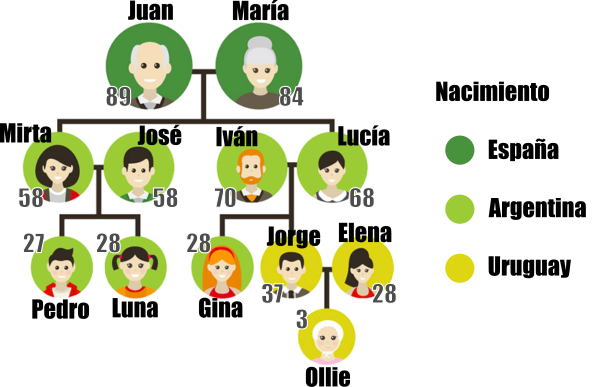
\includegraphics[height=5cm]{img/familia.png} \end{center}
	\begin{enumcols} 
		\item Verificar que la relación "$x$ tiene el mismo color de pelo que $y$" es una relación de equivalencia y representarla con un grafo. Indicar las clases de equivalencia y el conjunto cociente.
		\answer La relación es reflexiva, simétrica y transitiva. Las clases de equivalencia son $K_{\text{Juan}}=\{$Juan, María$\}$ (pelo gris), $K_{\text{Mirta}}=\{$Mirta, José, Lucía, Pedro, Luna, Jorje, Elena$\}$ (pelo negro), $K_{\text{Iván}}=\{$Iván, Gina$\}$ (pelo colorado) y $K_{\text{Ollie}}=\{$Ollie$\}$ (pelo blanco). El conjunto cociente es $\{K_{\text{Juan}}, K_{\text{Mirta}}, K_{\text{Iván}}, K_{\text{Ollie}}\}$

		\item Verificar que la relación "$x$ nació en el mismo país que $y$" es una relación de equivalencia y representarla con un grafo. Indicar las clases de equivalencia y el conjunto cociente.
		
		\item Verificar que la relación "$x$ es descendiente de $y$" es una relación de orden estricto parcial. Representar la relación en un diagrama de Hasse.
		
		\item Explicar porque la relación "$x$ es de la misma edad o mayor que $y$" NO ES una relación de orden amplio.
		\answer Porque no es antisimétrica. (Mirta)$\mathrel{R}$(José) $\land$ (José)$\mathrel{R}$(Mirta) pero José$\neq$Mirta. También se puede verificar con Luna, Gina y Elena, que tienen la misma edad.
	
	\end{enumcols}

	\exercise Resolver los siguientes ejercicios variados
	\begin{enumcols}

		\item Sean $R_1$ y $R_2$ dos relaciones de equivalencia en $A$. Averiguar si $R_1 \intersec R_2$ y $R_1 \union R_2$ son relaciones de equivalencia en $A$.
		\answer $R_1 \intersec R_2$ es de equivalencia mientras que $R_1 \union R_2$ no lo es necesariamente.

		\item Sea $R$ una relación definida en el conjunto de número reales tal que $x R y \Eq |x-y|<1$. Demostrar que $R$ no es una relación de equivalencia.
		\answer $R$ es reflexiva porque $|x - x| = 0 < 1$. \\ $R$ es simétrica ya que $|x - y|=|y - x|$ por lo que $|x-y|<1 ~\Then~ |y - x| < 1$. \\ $R$ NO es transitiva. Contraejemplo: $x = 2.8$, $y = 1.9$, y $z = 1.1$, donde se ve que $|2.8-1.9|=0.9<1$, $|1.9-1.1|=0.8<1$, pero $|2.8-1.1|=1.7>1$. \\ Por lo tanto, $R$ no es una relación de equivalencia.

		\item En $\Z$ se define la relación $R$ mediante: $(a,b) \in R \Eq a^2+a=b^2+b$. Clasificar $R$.

		\item En $\R^2$ se define la relación $\sim$ mediante: $(x,y) \sim (x',y') \Eq x=x'$. Probar que $\sim$ es de equivalencia, determinar las clases de equivalencia y el conjunto cociente.
		\answer Resolución por \href{https://youtu.be/AZCm7mr90eA?si=00bQgRjxNRtq0dgn&t=784}{La mano matemática}

		\item En $A=\{1,2,4,6,8\}$ se define la siguiente relación: $xRy \Eq 3|(x+y)$. Definir $R$ por extensión, clasificarla y realizar su gráfico o esquema.

		\item En $\N^2$ se define la siguiente relación: $(a,b)\sim(a',b') \Eq a+b'=a'+b$. Demostrar que es de equivalencia, obtener las clases de equivalencia, el conjunto cociente y representarla indicando las clases.
		\answer Resolución por \href{https://youtu.be/pcIquCFF8eY?si=4OyN1jYsMVnxr4sJ&t=1920}{Science and Tech}

		\item El conjunto $\{\{a\},\{b,c\},\{d\}\}$ es una partición de $A$. Obtener la relación de equivalencia asociada a la partición.

		\item En el conjunto $A=\{1,2,3,4,5\} \subseteq \N$ se considera la relación de menor o igual. Determinar, si los hubiere, los elementos maximales y minimales, el conjunto de cotas superiores e inferiores, y el supremo e ínfimo.

		\item En $\R$, ordenado por la relación de menor o igual, se define el conjunto $A=\left\{ x \in \R ~|~ x=\frac{1}{n} \land n\in \N \right\}$. Analizar si $A$ tiene primer y ultimo elemento, indicar el conjunto de cotas superiores, y analizar si el $0$ es una cota inferior.

		\item Sea $R$ una relación definida en el conjunto de personas tal que $xRy$ si y solo si $x$ es mayor (en edad) que $y$. Averiguar si $R$ es una relación de orden amplio/estricto total/parcial.

		\item Se define la relación $R$ en $\N$ de manera que $x R y \Eq \exists k \in \N: x=y.10^k$. Estudiar sus propiedades y clasificar la relación. En el caso de que sea de equivalencia dar las clases de equivalencia, en el caso de que sea de orden indicar si es parcial o total.
		\answer Resolución por \href{https://youtu.be/pcIquCFF8eY?si=MqmMft1L2whilZP0&t=973}{Science and Tech}.

		\item Sea $A=\{1,2,3,6,9,18\}$ y $R$ la relación en $A$ dada por $xRy \Eq x|y$, mostrar que es una relación de orden y trazar su diagrama de Hasse
		\answer Resolución por \href{https://youtu.be/YSBxulxpbVM?si=rW4cjcCnpCiS9wTy&t=365}{La mano matemática}  

		\item Definimos la relación $R$ en $\N$ por $xRy \Eq \f{x}{y}=2^n$ para algún $n\in\Z$. Verificar que es una relación de equivalencia y analizar si entre los números $1$, $2$, $3$ y $4$, hay algunos que pertenezcan a la misma clase de equivalencia.
		\answer Resolución por \href{https://youtu.be/AZCm7mr90eA?si=CfJoinl3shRZyfjO&t=1049}{La mano matemática}. 

	\end{enumcols}

	\exercise Dados los siguientes conjuntos (y sus superconjuntos asociados), obtener su máximo y mínimo, el conjunto de cotas superiores e inferiores, su supremo y su ínfimo.
	\begin{enumcols}
		\item $(0,1]$ con la relación $\leq$ definida en $\R$.
		\answer Cotas superiores: $[1,+\infty)$. Cotas inferiores: $(-\infty,0]$. Supremo: $1$. Ínfimo: $0$. Máximo: $1$. Mínimo: $0$.  
		\item $[-8,5]$ con la relación $\leq$ definida en $\R$.
		\answer Cotas superiores: $[5,+\infty)$. Cotas inferiores: $(-\infty,-8]$. Supremo: $5$. Ínfimo: $-8$. Máximo: $5$. Mínimo: $-6$.
		\item $(-8,5)$ con la relación $\leq$ definida en $\R$.
		\answer Cotas superiores: $[5,+\infty)$. Cotas inferiores: $(-\infty,-8]$. Supremo: $5$. Ínfimo: $-8$. No existe máximo ni mínimo.
		\item $\mathcal{P}(\{1,2,3\})$ con la relación $\subseteq$ definida en $\mathcal{P}(\{1,2,3,4\})$.
		\answer Cotas superiores: $\{\{1,2,3\}, \{1,2,3,4\}\}$. Supremo: $\{1,2,3\}$. La única cota inferior es $\emptyset$, por lo tanto también es el ínfimo. Máximo: $\{1,2,3\}$. Mínimo: $\emptyset$.
	\end{enumcols}

	\exercise Analizar en cada caso si la relación dada en el conjunto $A$ es de equivalencia. En caso de serlo, describir su conjunto cociente.
	\begin{enumcols}
		\item $A=\R$ con $xRy \Eq x-y \in \Q$
		\answer Resolución por \href{https://youtu.be/EV_hHIqiMBE?si=4IetkI46A2SBp846&t=777}{La mano matemática}
		\item $A=\Z$ con $xRy \Eq x-y$ es un entero par
		\answer Resolución por \href{https://youtu.be/EV_hHIqiMBE?si=4IetkI46A2SBp846&t=777}{La mano matemática}
		\item $A=\R$ con $xRy \Eq x.y >0$
		\answer Resolución por \href{https://youtu.be/EV_hHIqiMBE?si=4IetkI46A2SBp846&t=777}{La mano matemática}
		\item $A=\R$ con $xRy \Eq x.y \geq 0$
		\answer Resolución por \href{https://youtu.be/EV_hHIqiMBE?si=4IetkI46A2SBp846&t=777}{La mano matemática}
		\item $A=\{1,2,3,4,5,6\}$ con $xRy \Eq x=y \lor x+y=5$ 
		\answer Resolución por \href{https://youtu.be/EV_hHIqiMBE?si=4IetkI46A2SBp846&t=777}{La mano matemática}
	\end{enumcols}


\end{enumerate}

\end{document}